\chapter{Conclusion}
brief of conclusion

\section{Cokro Edi Prawiro / 1164069}

\subsection{Teori}
\begin{enumerate}

\item Jelaskan Kenapa Kata-Kata harus dilakukan vektorisasi lengkapi dengan ilustrasi gambar.\par
Kata kata harus dilakukan vektorisasi dikarenakan atau bertujuan utk mengukur nilai kemunculan suatau kata yang serupa dari sebuah kalimat sehingga kata-kata tersebut dapat di prediksi kemunculanya. atau juga di buatnya vektorisasi data digunakan untuk memprediksi bobot dari suatu kata misalkan ayam dan kucing sama-sama hewan maka akan dibuat prediksi apakah kata tersebut akan muncul pada kalimat yang kira-kira memiliki bobot yang sama. untuk dapat jelasnya dapat melihat ilustrasi pada gambar \ref{c71}.

\item Jelaskan Mengapa dimensi dari vektor dataset google bisa mencapai 300 lengakapi dengan ilustrasi gambar. \par
Dimensi dataset dari google bisa mencapai 300 karena dimensi dari vektor tersebut digunakan untuk membandingkan bobot dari setiap kata, misalkan terdapat kata dog dan cat pada dataset google tersebut setiap kata tersebut di buat dimensi vektor 300 untuk kata dog dan 300 dimensi vektor juga untuk kata cat kemudian kata tersebt di bandingkan bobot kesamaan katanya maka akan muncul akurasi sekitar 70 persen kesamaan bobot dikarenakan kata dog dan cat sama sama di gunakan untuk hewan priharaan. untuk lebih jelasnya dapat dilihat pada gambar \ref{c72}.

\item Jelaskan Konsep vektorisasi untuk kata . dilengkapi dengan ilustrasi atau gambar. \par
Vektorisasi untuk kata untuk mengetahui kata tengah dari suatau kalimat atau kata utama atau objek utama pada suatau kalimat contoh ( Jangan lupa subscribe channel saya ya sekian treimakasih ) kata tengah tersebut merupakan channel yang memiliki bobot sebagai kata tengah dari suatu kalimat atau bobot sebagai objek dari suatu kalimat. hal ini sangat berkaitan dengan dimensi vektor pada dataset google yang 300 tadi karena untuk mendapatkan nilai atau bobot dari kata tengah tersebut di dapatkan dari proses dimensiasi dari kata tersebut. untuk lebih jelasnya dapat dilihat pada gambar \ref{c73} berikut :

\item Jelaskan Konsep vektorisasi untuk dokumen. dilengkapi dengan ilustrasi atau gambar. \par
Vektorisasi untuk dokumen hampir sama seperti vektorisasi untuk kata hanya saja pemilihan kata utama atau kata tengah terdapat pada satu dokumen jadi mesin akan membuat dimensi vektor 300 untuk dokumen dan nanti kata tengahnya akan di sandingkan pada dokumen yany terdapat pada dokumen tersebut contoh dapat dilihat pada gambar \ref{c74} berikut : 

\item Jelaskan apa mean dan standar deviasi, lengkapi dengan iludtrasi atau gambar. \par
mean merupakan petunjuk terhadap kata-kata yang di olah jika kata kata itu akurasinya tinggi berarti kata tersebut sering muncul begitu juga sebaliknya untuk lebih jelasnya dapat dilihat pada gambar \ref{c75} sedangkan setandar defiation merupakan standar untuk menimbang kesalahan. sehingga kesalahan tersebut di anggap wajar misarkan kita memperkirakan kedalaman dari dataset merupakan 2 atau 3 tapi pada kenyataanya merupakan 5 itu merupakan kesalahan tapi masih bisa dianggap wajar karna masih mendekati perkiraan awal.

\item Jelaskan Apa itu Skip-Gram sertakan contoh ilustrasi. \par
Skip-Gram adalah kebalikan dari konsep vektorisasi untuk kata dimana kata tengah menjadi acuan terhadap kata kata pelengkap dalam suatu kalimat untuk lebih jelasnya dapat di lihat pada gambar \ref{c76} berikut :

\end{enumerate}

\begin{figure}
      \centerline{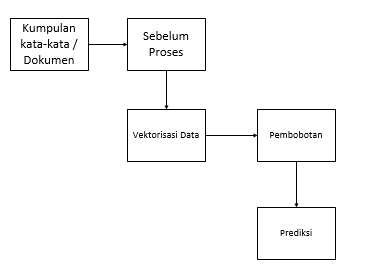
\includegraphics[width=1\textwidth]
      {figures/cokro/c71}}
      \caption{Ilustrasi Vektorisasi Kata-Kata}
      \label{c71}
      \end{figure}

\begin{figure}
      \centerline{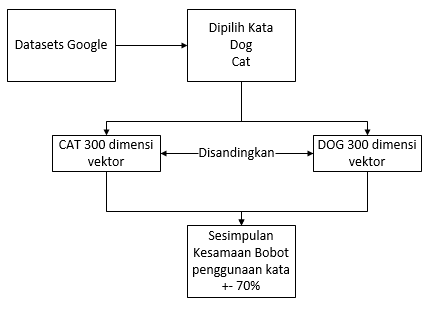
\includegraphics[width=1\textwidth]
      {figures/cokro/c72}}
      \caption{Ilustrasi Kenapa dimensi vektor pada datasets google haris 300}
      \label{c72}
      \end{figure}

\begin{figure}
      \centerline{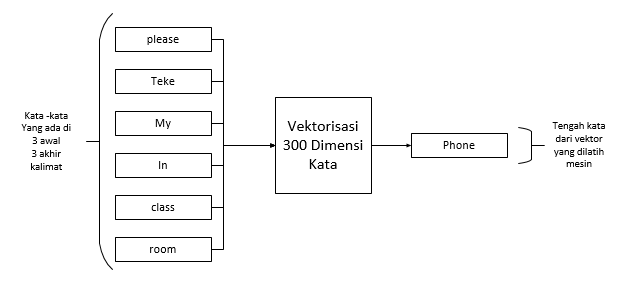
\includegraphics[width=1\textwidth]
      {figures/cokro/c73}}
      \caption{Ilustrasi konsep vektorisasi untuk kata}
      \label{c73}
      \end{figure}

\begin{figure}
      \centerline{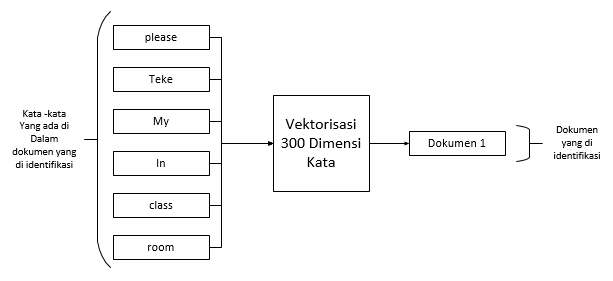
\includegraphics[width=1\textwidth]
      {figures/cokro/c74}}
      \caption{Ilustrasi konsep vektorisasi untuk dokumen}
      \label{c74}
      \end{figure}

\begin{figure}
      \centerline{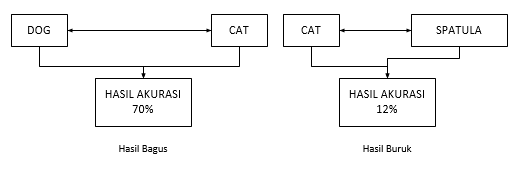
\includegraphics[width=1\textwidth]
      {figures/cokro/c75}}
      \caption{Ilustrasi Penggunaan Mean}
      \label{c75}
      \end{figure}


\begin{figure}
      \centerline{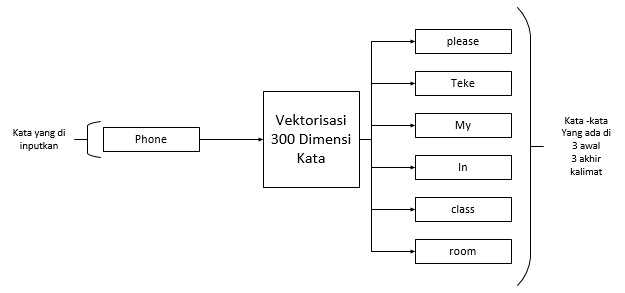
\includegraphics[width=1\textwidth]
      {figures/cokro/c76}}
      \caption{Ilustrasi Skip-Gram}
      \label{c76}
      \end{figure}